\documentclass[11pt,xcolor=table]{beamer}
\usetheme{CambridgeUS}
\usecolortheme{dolphin}

\usepackage[utf8]{inputenc}
\usepackage[L7x]{fontenc}
\usepackage[lithuanian]{babel}
\usepackage{lmodern} %be neveikia bold, italic etc


\usepackage{amsmath}
\usepackage{amsfonts}
\usepackage{amssymb}

\usepackage{graphicx}
\graphicspath{{./figures/}}

\usepackage{adjustbox}
\usepackage{bm}
\usepackage{subcaption}

\usepackage{multirow} % for multirow tables
\setbeamertemplate{caption}[numbered] % for numbering captions

\usepackage{forest}


\usepackage{listings}
\usepackage{color}
\usepackage{textcomp}
\definecolor{listinggray}{gray}{0.9}
\definecolor{lbcolor}{rgb}{0.9,0.9,0.9}
\lstset{
	backgroundcolor=\color{lbcolor},
	tabsize=4,
	rulecolor=,
	language=matlab,
        basicstyle=\scriptsize,
        upquote=true,
        aboveskip={0.5\baselineskip},
        belowskip={0.5\baselineskip},
        columns=fixed,
        showstringspaces=false,
        extendedchars=false,
        breaklines=true,
        prebreak = \raisebox{0ex}[0ex][0ex]{\ensuremath{\hookleftarrow}},
        frame=single,
        showtabs=false,
        showspaces=false,
        showstringspaces=false,
        identifierstyle=\ttfamily,
        keywordstyle=\color[rgb]{0,0,1},
        commentstyle=\color[rgb]{0.133,0.545,0.133},
        stringstyle=\color[rgb]{0.627,0.126,0.941}
}


\usepackage{tikz, pgfplots}
\usetikzlibrary{patterns,decorations.pathreplacing}


\author{Justas Mundeikis}
\title{Duomenų analizės įvadas}
%\setbeamercovered{transparent} 
%\setbeamertemplate{navigation symbols}{} 
%\logo{} 
%\institute{} 
%\date{} 
%\subject{} 



%----------------------------------------------------------
\begin{document}
%----------------------------------------------------------
\section{Apie kursą}
%----------------------------------------------------------

\begin{frame}
\titlepage
\end{frame}
%----------------------------------------------------------
\begin{frame}{Šio kurso turinys:}
\begin{enumerate}
\item Įvadas: apie kursą, CLI,  Git ir GitHub, R ir RStudio
\item R programavimo pagrindai
\item Tiriamoji duomenų analizė (angl.: exploratory data analysis)
\item Atkartojami tyrimai (angl.: reproducible research) su LaTex, RMarkdown, Jupyter
\end{enumerate}
\end{frame}
%----------------------------------------------------------
\begin{frame}{Kurso tikslas}

{\Large In God we trust, all others bring data}\\ 
{\scriptsize - W. Edwards Deming }

\begin{itemize}
\item Suteikti pagrindines reikalingas kompetencijas darbui su duomenimis
\item Šis kursas labiau taikomasis, nėra aiškios takoskyros tarp paskaitų ir seminarų
\item Kursas yra "lengvas", tačiau reikalauja daug praktinio darbo pastangų
\item Dirbama tik su R, RStudio, Git ir Github, Jupyter?
\item Neliesime Matlab, Python, Julia, Eviews
\item Laikas \textbf{savistudijoms}
\item Vietiniai PC vs. nuosavi notebook'ai
\end{itemize}
\end{frame}
%----------------------------------------------------------
\begin{frame}{Kurso vertinimo strategija}

\begin{itemize}
\item Savaitiniai namų darbai - 30\%
\\Savaitinių namų darbų tikslas parodyti studentams kokio pobūdžio uždavinius studentai turi gebėti savarankiškai spręsti. Namų darbų vertinimas: maksimumas iš leidžiamų 3 bandymų
\item Neanonsuoti testai - 30\%
\\Neanonsuoti trumpi testai skirti užtikrinti, jog studentai nuolatos skirtų deramą dėmesį ir laiku įdėtų reikalingas pastangas studijoms
\item Baigiamasis egzaminas - 40\%
\\Egzamine tikrinamos tiek teorijos tiek įgytos praktinės žinios 
\item $BP=ceiling(mean(SND)*0.3+mean(NT)*0.3+BE*0.4)$
\end{itemize}
\end{frame}
%----------------------------------------------------------
\begin{frame}{Sando pristatymas}
\begin{itemize}
\item Sando pristatymas
\item Klausimai?
\end{itemize}
\end{frame}

%----------------------------------------------------------
\section{Įvadas}
\begin{frame}{Įvadas į duomenų analizę, Git ir GitHub, R ir RStudio}
Šioje dalyje susipažinsime su
\begin{itemize}
\item CLI
\item Git 
\item Github
\item R 
\item RStudio
\end{itemize}
\end{frame}
%----------------------------------------------------------
\section{CLI}
%----------------------------------------------------------
\begin{frame}{Command Line interface (CLI)}
Kiekviena operacinė sistema turi CLI:
\begin{itemize}
\item Windows: Git Bash (), CMD
\item Mac/ Linux: Terminal'as
\end{itemize}
Su CLI galima:
\begin{itemize}
\item Naviguoti tarp aplankų (folder'ių)
\item Kurti, keisti, naikinti: failus, aplankus, programas
\item Startuoti programas
\end{itemize}
\end{frame}

%----------------------------------------------------------
\begin{frame}{Intarpas GIT Bash instaliavimas}
\begin{itemize}
\item Nors darbiniai kompiuteriai turi instaliuotą Git Bash, tiems kas neturi:
\item \href{https://git-scm.com/}{\textcolor{blue}{https://git-scm.com/}}
\item Windows 32/64, Linux žr. komandą
\item Perimti teikiamus standartinius siūlymus, nebent antrame Setup lange pasirinkti, jog Git Bash rodytų ir "Addditional icons: On the desktop"
\item startuojam Git Bash
\end{itemize}
\center
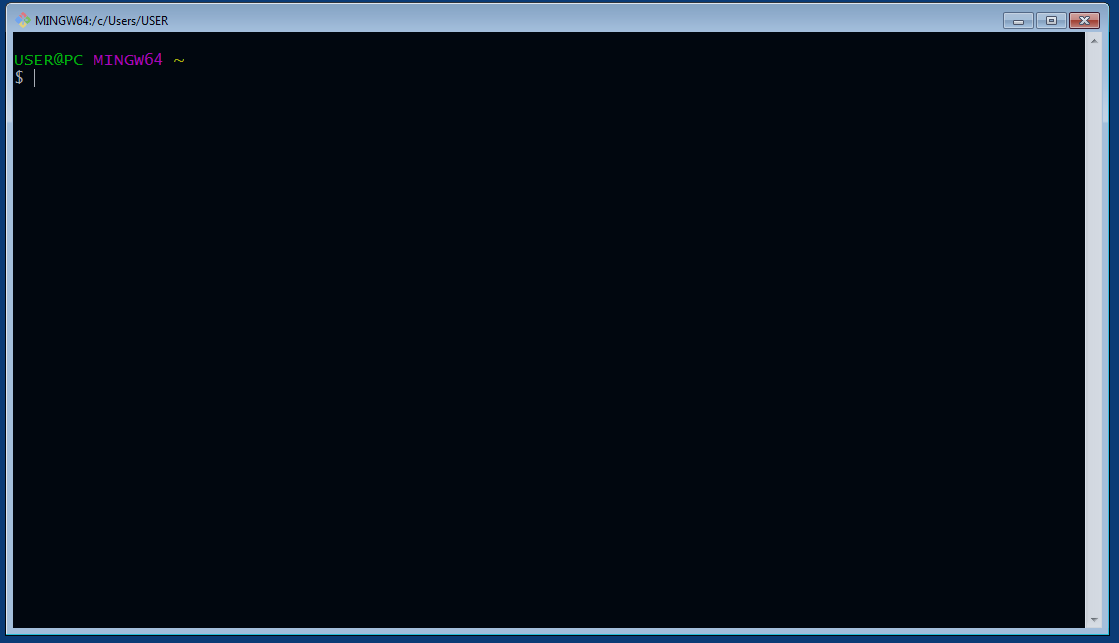
\includegraphics[scale=0.15]{Git_Bash_1.png}
\end{frame}
%----------------------------------------------------------
\begin{frame}{Direktorijos}
\begin{itemize}
\item "Directory" yra tiesiog kitas pavadinimas žodžiui aplankas
\item Direktorijos kompiuteryje organizuotos kaip medžio šakos
\item CLI padeda naviguoti tarp šių direktorijų
\item "/" yra root directory Linux, C: yra root directory Windows
\item root directory talpina visas kitas direktorijas
\end{itemize}
\center
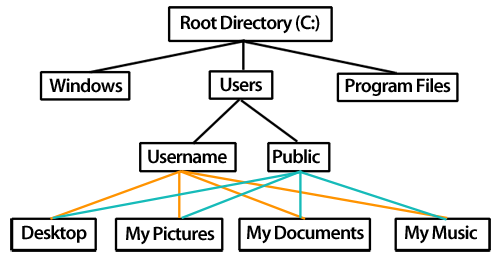
\includegraphics[scale=1.5]{diagram_directory_win.png}
\end{frame}

%----------------------------------------------------------
\begin{frame}[fragile]{Direktorijos}
\begin{itemize}
\item startavus matosi daug maž toks tekstas:

\begin{lstlisting}
USER@PC MINGW64 ~
$ 
\end{lstlisting}

\item \$ ženklas reiškia: "gali rašyti komandą"
\item tipinis įrašas: "command flag argument"
\item komandos pvz: komanda liepianti atspausdinti kurioje direktorijoje esama: "pwd"

\begin{lstlisting}
USER@PC MINGW64 ~
$ pwd
/c/Users/USER
\end{lstlisting}

\end{itemize}
\end{frame}

%----------------------------------------------------------
\begin{frame}[fragile]{Direktorijos}
\begin{itemize}
\item komanda gali būti iššaukiama su tam tikra programa
\item \colorbox{listinggray}{\lstinline|git init|}
\item \colorbox{listinggray}{\lstinline|python get-pip.py|}
\item flag: tam tikri nustatymai, galimi priklausomai nuo komandos ir visada su "-"
\item argument - kiti nustatymai, pakeitimai ar panašūs dalykai
\item \colorbox{listinggray}{\lstinline|git commit -m "this is the initial commit"|}
\item jeigu flag yra žodis , tada naudojami du brūkšniai -\/- 
\item \colorbox{listinggray}{\lstinline|git reset --hard HASH|}

\end{itemize}
\end{frame}

%----------------------------------------------------------
\begin{frame}{CLI komandos}
\begin{itemize}
\item "ls" nurodo visus failus ir folderius esančius direktorijoje
\item "ls -a" nurodo visus matomus ir paslėptus failus ir folderius
\item "ls -al" nurodo visų matomų ir paslėptų failų ir folderių detales
\item "clear" išvalo CLI
\end{itemize}
\end{frame}

%----------------------------------------------------------

\begin{frame}{CLI komandos}
\begin{itemize}
\item "cd"  reiškia "change directory"
\item "cd"  be argumentų sugrąžins į home directory
\item "cd .." pakels viena direktorija aukščiau
\item \textcolor{green}{Uždavinys: su cd nueiti and "Desktop"}
\end{itemize}
\end{frame}

%----------------------------------------------------------
\begin{frame}{CLI komandos}
\begin{itemize}
\item "mkdir" "make directory"  sukuria folderį pvz: "Duomenų analizės įvadas"
\item "rmdir" "remove directory", bet tik, jeigu folderis yra tuščias
\item \textcolor{green}{Nueiti į sukrtą direktoriją}
\item "touch" sukuria failą, pvz., "touch info.txt"
\item \textcolor{green}{Sukurti dvi direktorijas folder1 ir folder2}
\item "cp" kopijuoja failus (cp failas direktorija)
\item "cp failas failas" padaro failo kopiją
\item "cp info.txt folder1"
\item "cp -r" folderis direktorija (-r recursive t.y. įtraukia viską, kas yra folderio viduje)
\item "cp -r folder1 folder2"
\end{itemize}
\end{frame}

%----------------------------------------------------------
\begin{frame}{CLI komandos}
\begin{itemize}
\item "rm" "remove" su argumentu failo pavadinimu
\item "rm -r" su direktorijos pavadinimu viskam kas direktorijoje
\item "mw failas direktorija" perkelia failą (Cut+Paste)
\item "mv" failassenas failasnaujas (pakeičia pavadinimą) (Rename)
\item "echo" atspausdina tekstą (echo Labas; echo date)
\item "nano failas" startuoja nano editorių 
\item "exit" uždaro CLI 
\end{itemize}
\end{frame}

%----------------------------------------------------------
\section{Git ir GitHub}
%----------------------------------------------------------
\begin{frame}{Trumpas įvadas į Git}
\begin{quote}
"Git is a version-control system for tracking changes in computer files and coordinating work on those files among multiple people. It is primarily used for source-code management in software development,but it can be used to keep track of changes in any set of files. As a distributed revision-control system, it is aimed at speed, data integrity, and support for distributed, non-linear workflows"
\end{quote}
\href{https://en.wikipedia.org/wiki/Git}{\textcolor{blue}{https://en.wikipedia.org/wiki/Git}}
\end{frame}
%----------------------------------------------------------
\begin{frame}{Git}
\begin{quote}
"Git is a free and open source distributed version control system designed to handle everything from small to very large projects with speed and efficiency"
\end{quote}
\href{https://git-scm.com/}{\textcolor{blue}{https://git-scm.com/}}
%----------------------------------------------------------
\begin{itemize}
\item Sukurta Linux kurėjo Linus Torvalds
\item Populiariausias VCS
\item Viskas išsaugoma lokaliai
\item GIT naudojamas naudojant CLI
\item http://git-scm.com/downloads
\end{itemize}
\end{frame}

%----------------------------------------------------------
\begin{frame}[fragile]{Git pagrdiniai nustatymai}
\begin{itemize}
\item Kiekvienas išsaugojimas bus susietas su išsaugotu "user.name" ir "user.email"
\item Tai reikia padaryti tik vieną kartą (dirbant su savo PC), arba pasikeisti kaskart prisėdus prie svetimo pc
\end{itemize}
\begin{lstlisting}
$ git config --global user.name "Justas Mundeikis"
$ git config --global user.email mundeikis@gmx.de
$ git config --list
$ git config --global -l
$ git config --global core.pager cat 
# core.pager is made to cat (cat=content, printed on CLI)
\end{lstlisting}
\end{frame}
%----------------------------------------------------------
\begin{frame}{GitHub}
\begin{quote}
"GitHub  is a web-based hosting service for version control using Git. It is mostly used for computer code. It offers all of the distributed version control and source code management (SCM) functionality of Git as well as adding its own features. It provides access control and several collaboration features such as bug tracking, feature requests, task management, and wikis for every project"
\end{quote}
\href{https://en.wikipedia.org/wiki/GitHub}{\textcolor{blue}{https://en.wikipedia.org/wiki/GitHub}}

\begin{itemize}
\item "push" ir "pull" tarp lokalių ir internetinių repozitorijų
\item suteikia homepage vartotojo repozitorijoms
\item GitHub atlieka back-up funkciją lokalioms repozitorijoms
\item leidžia bendradarbiauti, dalintis projektais, gerinti kitų kodą ir t.t.
\item GitHub paskyros susikūrimas...
\end{itemize}
\end{frame}
%----------------------------------------------------------
\begin{frame}[fragile]{Git}
\begin{itemize}
\item Su Git-Bash nueiname į "Desktop", kur sukuriame direktoriją "Duomenu analizes ivadas Sxxxxx" kur Sxxxx pažymi studento ID (šiuo kompiuteriu naudosis ir kiti studentai..)
\item Šioje direktorijoje sukuriame dar vieną direktoriją "1 Ivadas"
\item Inicializuojame git
\begin{lstlisting}
$ git init
Initialized empty Git repository in C:/Users/USER/Desktop/Duomenu analizes ivadas Sxxx/1 Ivadas/.git/
\end{lstlisting}
\item direktorijoje sukuriamas nematomas failas .git
\end{itemize}
\end{frame}
%----------------------------------------------------------
\begin{frame}{Git kaip foto sesija}
\begin{itemize}
\item GIT daro tarsi nuotraukas, pasirinktos direktorijos
\item inicializavimas, tai tarsi foto kambario pasirinkimas, kuriame gali būti daug "veikėjų"
\item "git add failas" yra tarsi "veikėjo" užvedimas ant foto scenos
\item "git commit" yra pačios nuotraukos darymas
\item tam kad nuotraukoje nebūtų tam tikrų asmenų galia naudoti sąrašą kuris slepiasi ".gitignore" faile
\end{itemize}
\center
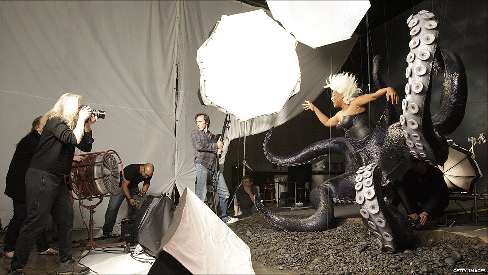
\includegraphics[scale=0.4]{photo_session.png}
\end{frame}


%----------------------------------------------------------

\begin{frame}[fragile]{Git}
\begin{itemize}
\item su komanda touch sukuriame failą readme.txt
\item "notepad readme.txt" įrašome change1, išsaugome 
\item šis failas egzistuoja direktorijoje, tačiau nėra "sekamas"
\begin{lstlisting}
$ git status
On branch master

No commits yet

Untracked files:
  (use "git add <file>..." to include in what will be committed)

        readme.txt

nothing added to commit but untracked files present (use "git add" to track)
\end{lstlisting}
\item Taigi failas readme.txt yra "untracked"
\end{itemize}
\end{frame}
%----------------------------------------------------------


\begin{frame}[fragile]{Git}
\begin{itemize}
\item su komanda "git add readme.txt" įkeliama readme.txt į staging area
\begin{lstlisting}
$ git status
On branch master

No commits yet

Changes to be committed:
  (use "git rm --cached <file>..." to unstage)

        new file:   readme.txt

\end{lstlisting}
\item Taigi failas reamde.txt yra staged bet dar ne "commited"
\item Ką reiškia, jog failas yra staged?
\end{itemize}
\end{frame}
%----------------------------------------------------------


\begin{frame}[fragile]{Git}
\begin{itemize}
\item notepad kitoje eilutėje įrašome "change2", išsaugome
\begin{lstlisting}
$ git status
On branch master
No commits yet
Changes to be committed:
  (use "git rm --cached <file>..." to unstage)

        new file:   readme.txt

Changes not staged for commit:
  (use "git add <file>..." to update what will be committed)
  (use "git checkout -- <file>..." to discard changes in working directory)

        modified:   readme.txt
\end{lstlisting}
\item dabar matome, jog readme.txt yra "tracked" ir "untracked"
\item Staging area esantis failas "readme.txt" yra išsaugotas tik su įrašu "change1", bet be su įrašu "change2"
\end{itemize}
\end{frame}
%----------------------------------------------------------

\begin{frame}[fragile]{Git}
\begin{itemize}
\item norint išsaugoti naujausią versiją: "git add readme.txt"
\item norint perduoti failą repozitorijai
\begin{lstlisting}
$ git commit -m "sukurtas failas readme.txt"

[master (root-commit) 30cd9e9] sukurtas failas readme.txt
 1 file changed, 1 insertion(+)
 create mode 100644 readme.txt
\end{lstlisting}
\item dabar patikrinus statusą
\begin{lstlisting}
$ git status
On branch master
nothing to commit, working tree clean
\end{lstlisting}
\end{itemize}
\end{frame}
%----------------------------------------------------------

\begin{frame}[fragile]{Git}
\begin{itemize}
\item readme.txt prirašome "change3", stagindam ir commitiname su -m "sukurtas change3"
\end{itemize}
\end{frame}

%----------------------------------------------------------
\begin{frame}[fragile]{Git}
\begin{itemize}
\item norint žinoti kas kada kaip keitė failą: "git log"
\item pateiktas log'as kiekvienam atrodys kitaip, bet esmė ta pati:
\begin{lstlisting}
$ git log
commit 1077a8e2e27424339d56a2dfd20b4aec56b0d3fb (HEAD -> master)
Author: Justas Mundeikis <mundeikis@gmx.de>
Date:   Tue Jan 1 07:19:02 2019 -0800

    sukurtas failas readme.txt

commit 30cd9e9503f37bc748de35ff66d2fae8d01e3d72
Author: Justas Mundeikis <mundeikis@gmx.de>
Date:   Tue Jan 1 07:16:54 2019 -0800

    sukurtas change3

\end{lstlisting}
\end{itemize}
\end{frame}

%----------------------------------------------------------

\begin{frame}[fragile]{Git}
\begin{itemize}
\item su touch sukuriame kitą failą "basic.R"
\item o readme.txt įrašome "change4"
\item "git status" parodo, jog pkaeistas readme.txt failas, ir untracked basic.R failas
\item su komanda "git add ." staginame visus failus
\item galimi kiti variantai : git stage -A, git stage -u (naudojamas tik update'inti esamus failus)
\item tada git commit -m "sukurtas change4 ir sukurtas faials basic.R"
\end{itemize}
\end{frame}
%----------------------------------------------------------

\begin{frame}[fragile]{Git}
\begin{itemize}
\item kartais yra tam tikri failai, kurių nenorime sekti (pvz duomenys, nereikalingi LaTex failai ir t.t.)
\item touch data.csv
\item git status parodo failą kaip untracked
\item todėl sukuriame faila .gitignoe ir jame įrašome failų pavadinimus, arba galūnes kurių nenorime trackinti
\begin{lstlisting}
git touch .gitignore
notepad .gitignore
\end{lstlisting}
\item atsidariusme editoriuje įrašome 
\begin{lstlisting}
*.csv 
\end{lstlisting}
\item * reiškia bet kokį pavadinimą, po kurio seka taškas ir csv, alternatyviai galima specifikuoti konkretų failą "data.csv"
\item "git status" neberodo failo "data.csv" bet rodo ".gitignore", todėl staginame ir commitiname pakeitimus
\end{itemize}
\end{frame}
%----------------------------------------------------------

\begin{frame}[fragile]{Git branch'inimas}
\begin{itemize}
\item Bazinis scenarijus:
\begin{itemize}
\item A kuria projektą, B nori prisidėti, tačiau ir A dirba tuo pat metu...
\item B atsiskelia atšaką (brach'ina) A projektą, padaro savo pakeitimus ir pateikia A juos sujungti
\item A peržiūri pakeitimus, priima/atmeta
\end{itemize}
\end{itemize}
\end{frame}

\begin{frame}[fragile]{Git branch'inimas}
\begin{itemize}
\item "git branch NewBranch" sukuria naują atšaką pavadinimu NewBranch
\item "git checkout NewBranch" išmeta iš "master" į "NewBranch"
\item atitinkmai "git choeckout master" visada sugrąžina atgal į master atšaką

\begin{lstlisting}
USER@PC MINGW64 ~/Desktop/Duomenu analizes ivadas Sxxx/1 Ivadas (master)
$ git branch NewBranch

USER@PC MINGW64 ~/Desktop/Duomenu analizes ivadas Sxxx/1 Ivadas (master)
$ git checkout NewBranch
Switched to branch 'NewBranch'

USER@PC MINGW64 ~/Desktop/Duomenu analizes ivadas Sxxx/1 Ivadas (NewBranch)

\end{lstlisting}

\item dabar visi pakeitimai vyks tik šioje atšakoje ir nepaveiks master šakos
\end{itemize}
\end{frame}
%----------------------------------------------------------

\begin{frame}{Darbas Git atšakoje}
\begin{itemize}
\item sukuriame naują faila "touch advanced.R"
\item readme.txt įrašome papildomą eilutę "change5"
\item staginti ir commitinti pakeitimus
sugrįžtame į master atšaką "git chekcout master"
\item Rezultatas: trūksta advanced.R failo, readme.txt turi tik 4 įrašus!
\item norint sujungti naują atšaką į master "git merge NewBranch"
\end{itemize}
\end{frame}
%----------------------------------------------------------

\begin{frame}[fragile]{Merge problemos}
\begin{itemize}
\item master branch readme.txt sukuriame eilute "change6", addinam ir commitiname (jeigu nesukurti nauji failai: git add -a -m "...")
\item nueiname į atšaką NewBranch, ir ten esančiame faile sukuriame change7, addinam ir commitiniame
\item grįžtame į master branch "git chekckout master"
\item ir bandome sujungti "git merge NewBranch"

\begin{lstlisting}
$ git merge NewBranch
Auto-merging readme.txt
CONFLICT (content): Merge conflict in readme.txt
Automatic merge failed; fix conflicts and then commit the result.
\end{lstlisting}
\item git negalėjo automatiškai sutvarkyti failų, todėl atsidarome readme.txt failą ir tvarkome patys
\end{itemize}
\end{frame}
%----------------------------------------------------------

\begin{frame}[fragile]{Konfliktinio failo tvarkymas}
\begin{itemize}
\item Atsidarius readme.txt matome

\begin{lstlisting}
change1
change2
change3
change4
change5
<<<<<<< HEAD
change6
=======
change7
>>>>>>> NewBranch
\end{lstlisting}
\item $<<<<<HEAD$ yra tai kas yra aktyvioje atšakoje
\item $>>>>NewBranch$ yra kas ateina iš sujungiamos atšakos
\item atskirta ======
\end{itemize}
\end{frame}

%----------------------------------------------------------

\begin{frame}[fragile]{Konfliktinio failo tvarkymas}
\begin{itemize}
\item Sutvarkome failą, taip kaip norime
\begin{lstlisting}
change1
change2
change3
change4
change5
change6
change7
\end{lstlisting}
\item saviname, ir tada "git commit -a -m "sujungtas failas iš NewBranch bei pašalintas konfliktas"
\item Yra papildomų įrankių, kurie padeda atlikti merge'inimo darbus, nes dažniausiai konfliktų visada bus
\end{itemize}
\end{frame}
%----------------------------------------------------------

\begin{frame}[fragile]{Konfliktinio failo tvarkymas}
\begin{itemize}
\item master atšakoje sukuriame failą "touch markdnwon.md", 
\item readme.txt papildome įrašu "error entry"
\item jeigu failo nestaginame ir necommitiname (nes pvz reikia trumpam kažką pakeisti kitoje atšakoje), ir periname į kitą atšaką, failas lieka o tai gali sukurti ateityje daug problemų
\item todėl  "git add ."
\item "git stach" nukelia ne commitintą failą į stached area. Failo neberodo darbalaukyje
\item dabar galime darbuotis kitose atšakose ir vėl grįžus: "git stach apply" ir markdown.md failas vėl atsiranda baigus ji taisyti, galima commitinti.
\item tai ir padarome
\end{itemize}
\end{frame}

%----------------------------------------------------------

\begin{frame}[fragile]{Git atsatatymas 1}
\begin{itemize}
\item Na štai po vidurnakčio pasidarbavus, padarėme klaidą:
\item readme.txt papildome įrašu "error entry" 
\item \colorbox{listinggray}{\lstinline|git commit -a -m "padarme klaida|}
\item Tarkime kažką sugadinome, bet žinome, jog versija prieš tai veikė gerai
\item su "git log" susirandame "blogo" commit hashą  pvz 123456
\item \colorbox{listinggray}{\lstinline|git log --oneline|} pateikia logą trumpąją versiją
\item komanda \colorbox{listinggray}{\lstinline|git revert HASH|} atstato pasirinktą versiją, versijos su "error entry" nebėra!
\item po įvedimo "git revert hash" atsiranda langas, message langas (atitinka -m "...."), nes revert'inimas yra naujas commit
\end{itemize}
\end{frame}

%----------------------------------------------------------


\begin{frame}[fragile]{Git atsatatymas 2}
\begin{itemize}
\item Tarkime jus labai daug darbavotės, turite n commit padarę ir surpatote, kad pirmas commit buvo geras, o po to viskas ne.
\item "git reset --hard hash" komanda padaro hard-reset, t.y. resetina į pasirinktą commitą, tačiau ištrina viską, kas buvo daryta po to!
\item revert'inti \colorbox{listinggray}{\lstinline|git reset --hard HASH|} neįmanoma, priešingai nei paties revert.
\end{itemize}
\end{frame}

%----------------------------------------------------------

\begin{frame}{Git remote}
\begin{itemize}
\item norint žinoti, ar lokali repozitorija yra susieta su nuotoline repozitorija (pvz Github, Bitbucket ar pan)
\item \colorbox{listinggray}{\lstinline|git remote|}
\end{itemize}
\end{frame}

%----------------------------------------------------------

\begin{frame}
\begin{itemize}
\item Nueiname kiekvienas į savo github ir ten susikuriame repo:
\begin{itemize}
\item pavadinimas: test-repo
\item Description paliekam tučią
\item inicializuojame su 
\end{itemize}
\item Git Bash lange pakylame viena direktorija aukščiau, lauk iš "1 Įvadas" folderio su \colorbox{listinggray}{\lstinline|cd ..|}
\item GitHub nusikopijuojame sukurtos repo HTPPS adresą
\item Git Bash  įrašome \colorbox{listinggray}{\lstinline| git clone HTTPS|}
\item Dabartinėje direktorijoje atsirado test-repo folderis, keliaujame į jį \colorbox{listinggray}{\lstinline| cd "test-repo"|} 
\item \colorbox{listinggray}{\lstinline|git remote|}
\item \colorbox{listinggray}{\lstinline|git remote -v|} parodo HTTPS
\end{itemize}
\end{frame}

%----------------------------------------------------------

\begin{frame}{Git repo klonavimas}
\begin{itemize}
\item Klonavimas reiškia, jog mes sukuriame remote repo kloną savo kompiuteryje, su visa Git istorija.
\item Tarkime tai ne mūsų remote repo ir po klonavimo me skurį laiką nieko nedarėme. Galbūt tuo metu  originalo autorius kažką pakeite, tada galima
\item \colorbox{listinggray}{\lstinline|git fetch origin|}
\item Tai persiunčia pakeitimus, bet nemerge'ina
\item \colorbox{listinggray}{\lstinline|git remote pull origin|}
\item atitinka fetch+merge
\end{itemize}
\end{frame}

%----------------------------------------------------------

\begin{frame}{Git repo klonavimas}
\begin{itemize}
\item Sukurkime test-repo direktorijoje naują failą
\item \colorbox{listinggray}{\lstinline|touch info.txt|}
\item \colorbox{listinggray}{\lstinline|notepad info.txt |} prirašome ko nors, išsaugome
\item \colorbox{listinggray}{\lstinline|git add info.txt|}
\item \colorbox{listinggray}{\lstinline|git commit -m "pridetas info.txt failas"|}
\item dabar galime push'inti lokalius pakeitimus į github:
\item \colorbox{listinggray}{\lstinline|git push origin |}
\item pareikalavus įrašome github username ir userpassword
\item GitHub atnaujiname (F5) ir voila, failas info.txt yra remote repozitorijoje
\end{itemize}
\end{frame}

%----------------------------------------------------------

\begin{frame}{Lokalios repo sukėlimas į remote repo}
\begin{itemize}
\item Nueiname kiekvienas į savo GitHub ir ten susikuriame repo:
\begin{itemize}
\item pavadinimas: test-repo2
\item Description paliekam tučią
\item NE inicializuojame su README!!!!
\end{itemize}
\item keliaujame į savo "1 Įvadas" direktopriją
\item \colorbox{listinggray}{\lstinline|git remote add origin HTPPS"|}
\item \colorbox{listinggray}{\lstinline|git push origin master|}
\end{itemize}
\end{frame}

%----------------------------------------------------------

\begin{frame}
\begin{itemize}
\item Yra du metodai kaip sukurti GitHub repozitoriją
\begin{enumerate}
\item Tiesiog sukurti naują repozitoriją
\item "Fork" ("šakutinti") kito GitHub vartotojo jau egzistuojančią repozitoriją
\end{enumerate}
\end{itemize}
\end{frame}

%----------------------------------------------------------
\section{Markdown sintaksė}
%----------------------------------------------------------
\begin{frame}[fragile]{Markdown sintaksė}
\begin{itemize}
\item GitHub sukuriant repo, ją galima inicijuoti su readme.md
\item .md reiškia, jog tai yra markdown formatas
\item Markdown is a lightweight markup language with plain text formatting syntax. Its design allows it to be converted to many output formats, but the original tool by the same name only supports HTML. Markdown is often used to format readme files, for writing messages in online discussion forums, and to create rich text using a plain text editor. (\href{https://en.wikipedia.org/wiki/Markdown}{\textcolor{blue}{https://en.wikipedia.org/wiki/Markdown}})
\item Labai trumpa pagalba dėl formatavimo: \href{https://commonmark.org/help/}{\textcolor{blue}{https://commonmark.org/help/}}
\item Vėliau mes susipažinsime su RMarkdown
\end{itemize}
\end{frame}
%----------------------------------------------------------


\section{R}
%----------------------------------------------------------

\begin{frame}[fragile]{R paketai}
\begin{itemize}
\item dauguma R paketų saugomi CRAN (Comprehensive R Archive Network), iš kur atsisiunčiamas ir pats R
\item basinė R versija turi tik keletą naudingų paketų
\item available.packages() funkcija, kuri surenką visą informaciją apie ezistuojančius R paketus @CRAN
\begin{lstlisting}
a <- available.packages()
length(a)
\end{lstlisting}
\item Šiuo metu : 228140 paketai
\item taip pat galima ir iš github
\item install.packages("ggplot")
\item  install.packages(c("ggplot", "dplyr"))
\item iš R 
\item library(ggplot) čia nebereikia kabučių!
\item search() parodo visus įjungtus paketus
\end{itemize}
\end{frame}
%----------------------------------------------------------
\begin{frame}{R ir RStudio instaliavimas}
\begin{itemize}
\item R reikia instaliuoti iš CRAN
\item \href{https://cran.r-project.org/}{\textcolor{blue}{https://cran.r-project.org/}}
\item Paleidžiame R 
\item Tam kad būtų lengviau dirbti su R, turėti aibę papildomų funkcijų, instaliuojame RStudio
\item \href{https://www.rstudio.com/products/rstudio/download/}{\textcolor{blue}{https://www.rstudio.com/products/rstudio/download/}}
\item Startuojame RStudio
\end{itemize}
\end{frame}
%----------------------------------------------------------

\begin{frame}
\begin{itemize}
\item Aprašomoji 
\item Tiriamoji
\item Inferencinė
\item Progozuojamoji
\item Pražastiniai ryšiai
\item Mechanistinė
\end{itemize}
\end{frame}
%----------------------------------------------------------
\begin{frame}
Aprašyti duomenis
\begin{itemize}
\item Įprastai pirma statistinė analizė, kuri atliekama
\item Nedaromos jokios išvados ar prognozės
\item https://osp.stat.gov.lt/pagrindiniai-salies-rodikliai
\item https://osp.stat.gov.lt/statistika-vizualiai
\end{itemize}
\end{frame}
%----------------------------------------------------------
\begin{frame}
Tiriamoji analizė
\begin{itemize}
\item Naudojama aptikti sąsajoms tarp duomenų
\item Padeda rasti kelią kuriuo galima judėti tyrime pirmyn
\item EDA nenaudojama generalizuojant ar prognozuojant
\item "Correlation does not imply causation"
\end{itemize}
\end{frame}

\begin{frame}
Tikslas: naudojant maža dalį duomenų daryti išvadas apie bendrą populiaciją
\begin{itemize}
\item Inferencinė analizė - statistikos pagrindas
\item Taikant inferencinę analizę siekiama nustatyti dominantį kiekį bei su prognoze susijusią paklaidą
\end{itemize}
\end{frame}
%----------------------------------------------------------

\begin{frame}
Naudojant turimą informaciją apie tam tikrus opbjektus prognozuoti reikmšes kitiems objektams
\begin{itemize}
\item Jeigu X prognozuoja Y nereiškia, kad X iššaukia Y
\item Prognozavimo taiklumas priklauso nuo teisingo matuojamų kintamųjų pasirinkimo
\item Kuo daugiau duomenų ir kuo paprastesnis modelis!
\item Fivethirthyeigh.blogs.nytimes.com 
\item AMAZON pirkiniai
\item Reklama
\end{itemize}
\end{frame}
%----------------------------------------------------------
\begin{frame}
Kas nutika vienam kitntamajam, kai pakeičiamas kitas kintamasis
\begin{itemize}
\item Reikalingos randomizuotos studijos
\item Yra būdų kaip tai apeiti (ekonometrika magistre / PhD)
\item Dažniausiai gaunami vidutiniai efektai
\item Aksinis standartas
\item MMA ....
\end{itemize}
\end{frame}
%----------------------------------------------------------
\begin{frame}
Mechanistinė analizė: kaip ir kokie būtent pokyčiai vieno kintamojo keičia daro įtaką kitiems kintamiesiems (fizikos/inžinerijos sritis)
\end{frame}
%----------------------------------------------------------

\begin{frame}{Duomenys}
\begin{quote}
"Data are values of qualitative or quantitative variables, belonging to a set of items"
\end{quote}
wiki/data
Kokybiniai: Šalis, lytis, vardas
Kiekybiniai: Aukštis, svoris, spaudimas, kiekis
\end{frame}
%----------------------------------------------------------
\begin{frame}{Kaip atrodo duomenys?}
PAV, html, csv
\end{frame}
%----------------------------------------------------------
\begin{frame}
\begin{itemize}
\item Svarbiausias aspektas - klausimas
\item Antras pagal svarbumą - duomenys
\item Dažnai duomenys apribos arba išlaisvins Jus, bet tik duomenys be klausimo, neišgelbės
\end{itemize}
\end{frame}
%----------------------------------------------------------
\begin{frame}{Big Data}
\begin{itemize}
\item Travers and Milgram 1696 Sociometry
\item Leskovec and Horvitz WWW'08
\item Dont use hadoo your data isnt that big
\item "The data may not contain the asnwer. The combination of some data and an aching desire for an answer does not ensure that a reasonable answer can be extracted from a given body of data.." -  John Tukey
\end{itemize}
\end{frame}
%----------------------------------------------------------

%----------------------------------------------------------
\end{document}